\subsubsection{Fase complessiva}

\myparagraph{Prospetto orario}
In questa fase, la distribuzione oraria dei componenti del gruppo è la seguente:

{

\rowcolors{2}{azzurro2}{azzurro3}

\centering
\renewcommand{\arraystretch}{1.8}
\begin{longtable}{C{4cm} C{1cm} C{1cm} C{1cm} C{1cm} C{1cm} C{1cm} C{2cm}}

\rowcolor{azzurro1}
\textbf{Nominativo} &
\textbf{RE}&
\textbf{AM}&
\textbf{AN}&
\textbf{PT}&
\textbf{PR}&
\textbf{VE}&
\textbf{Ore totali}\\
\endhead

\MB & 0 & 0 & 0 & 5 & 4 & 11 & 20 \\
\VAS & 5 & 0 & 0 & 0 & 5 & 10 & 20 \\
\FD & 0 & 0 & 0 & 5 & 6 & 9 & 20 \\
\NM & 0 & 3 & 0 & 0 & 5 & 12 & 20 \\
\SB & 0 & 7 & 0 & 0 & 3 & 10 & 20 \\
\GB & 0 & 5 & 0 & 0 & 8 & 7 & 20 \\
\MDI & 10 & 0 & 0 & 6 & 0 & 4 & 20 \\
\textbf{Ore Totali} & 15 & 15 & 0 & 16 & 31 & 63 & 140 \\

\rowcolor{white}
\caption{Distribuzione oraria della fase di validazione e collaudo}\\

\end{longtable}
}
\newpage
Il seguente istogramma riassume i dati ottenuti:

\begin{figure}[H]
\centering
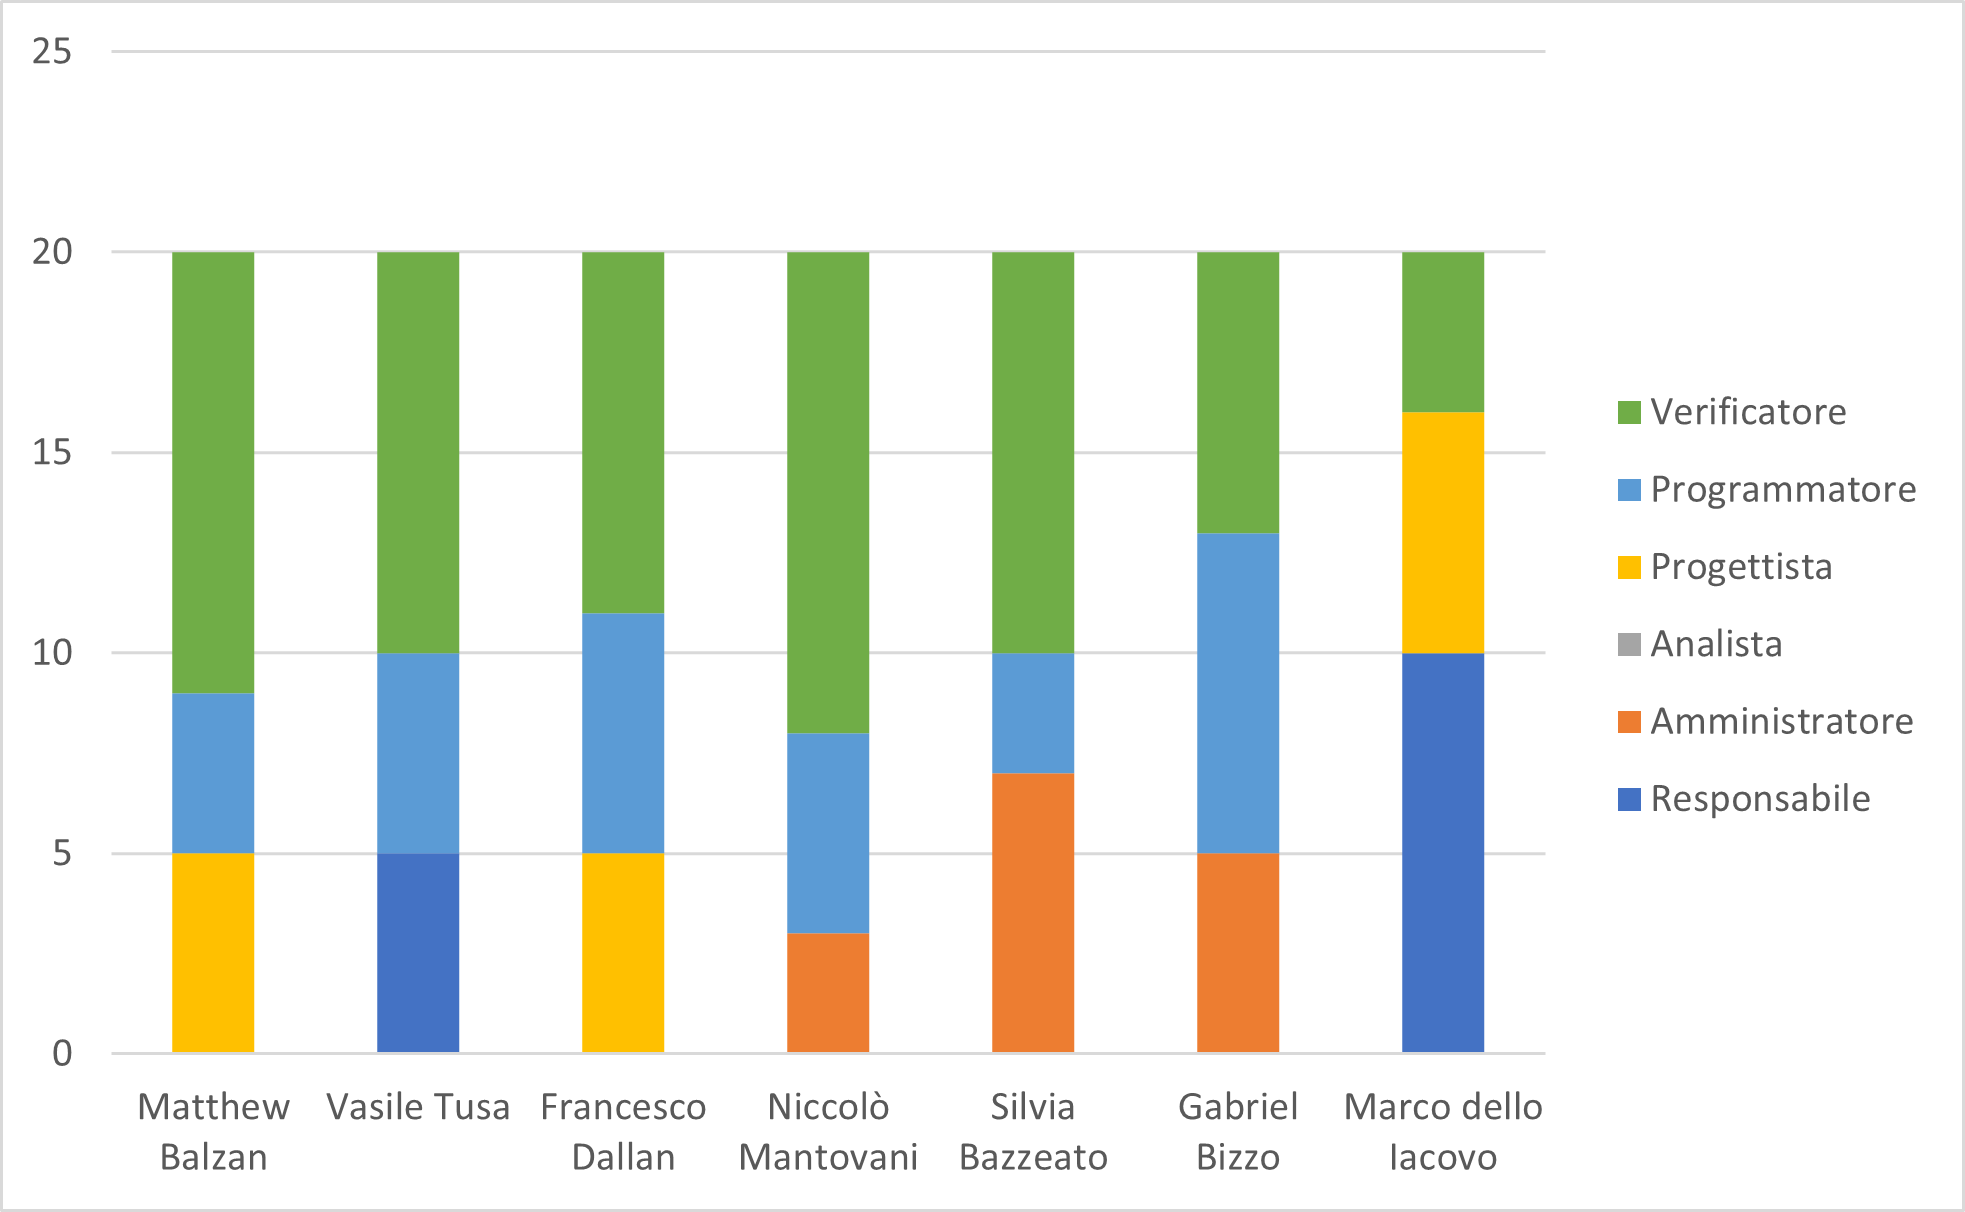
\includegraphics[scale=0.90]{res/Preventivo/Fasi/VerificaIncrementi/istogrammaFase}\\
\caption{Istogramma della ripartizione dei ruoli nella fase di validazione e collaudo}
\end{figure}


\myparagraph{Prospetto economico}

In questa fase, il costo per ogni ruolo è il seguente:

{

\rowcolors{2}{azzurro2}{azzurro3}

\centering
\renewcommand{\arraystretch}{1.8}
\begin{longtable}{C{3cm} C{1cm} C{2cm} }

\rowcolor{azzurro1}
\textbf{Ruolo} &
\textbf{Ore}&
\textbf{Costo}\\
\endhead

\textit{Responsabile} & 15 & 450\euro{} \\
\ammProg & 15 & 300\euro{} \\
\analProg & 0 & 0\euro{} \\
\progetProg & 16 & 352\euro{} \\
\programProg & 31 & 465\euro{} \\
\verifProg & 63 & 945\euro{} \\
\textbf{Totale} & 140 & 2512\euro{} \\

\rowcolor{white}
\caption{Prospetto dei costi per ruolo nella fase di validazione e collaudo}\\

\end{longtable}
}
\newpage
Il seguente areogramma riassume i dati ottenuti:

\begin{figure}[H]
\centering
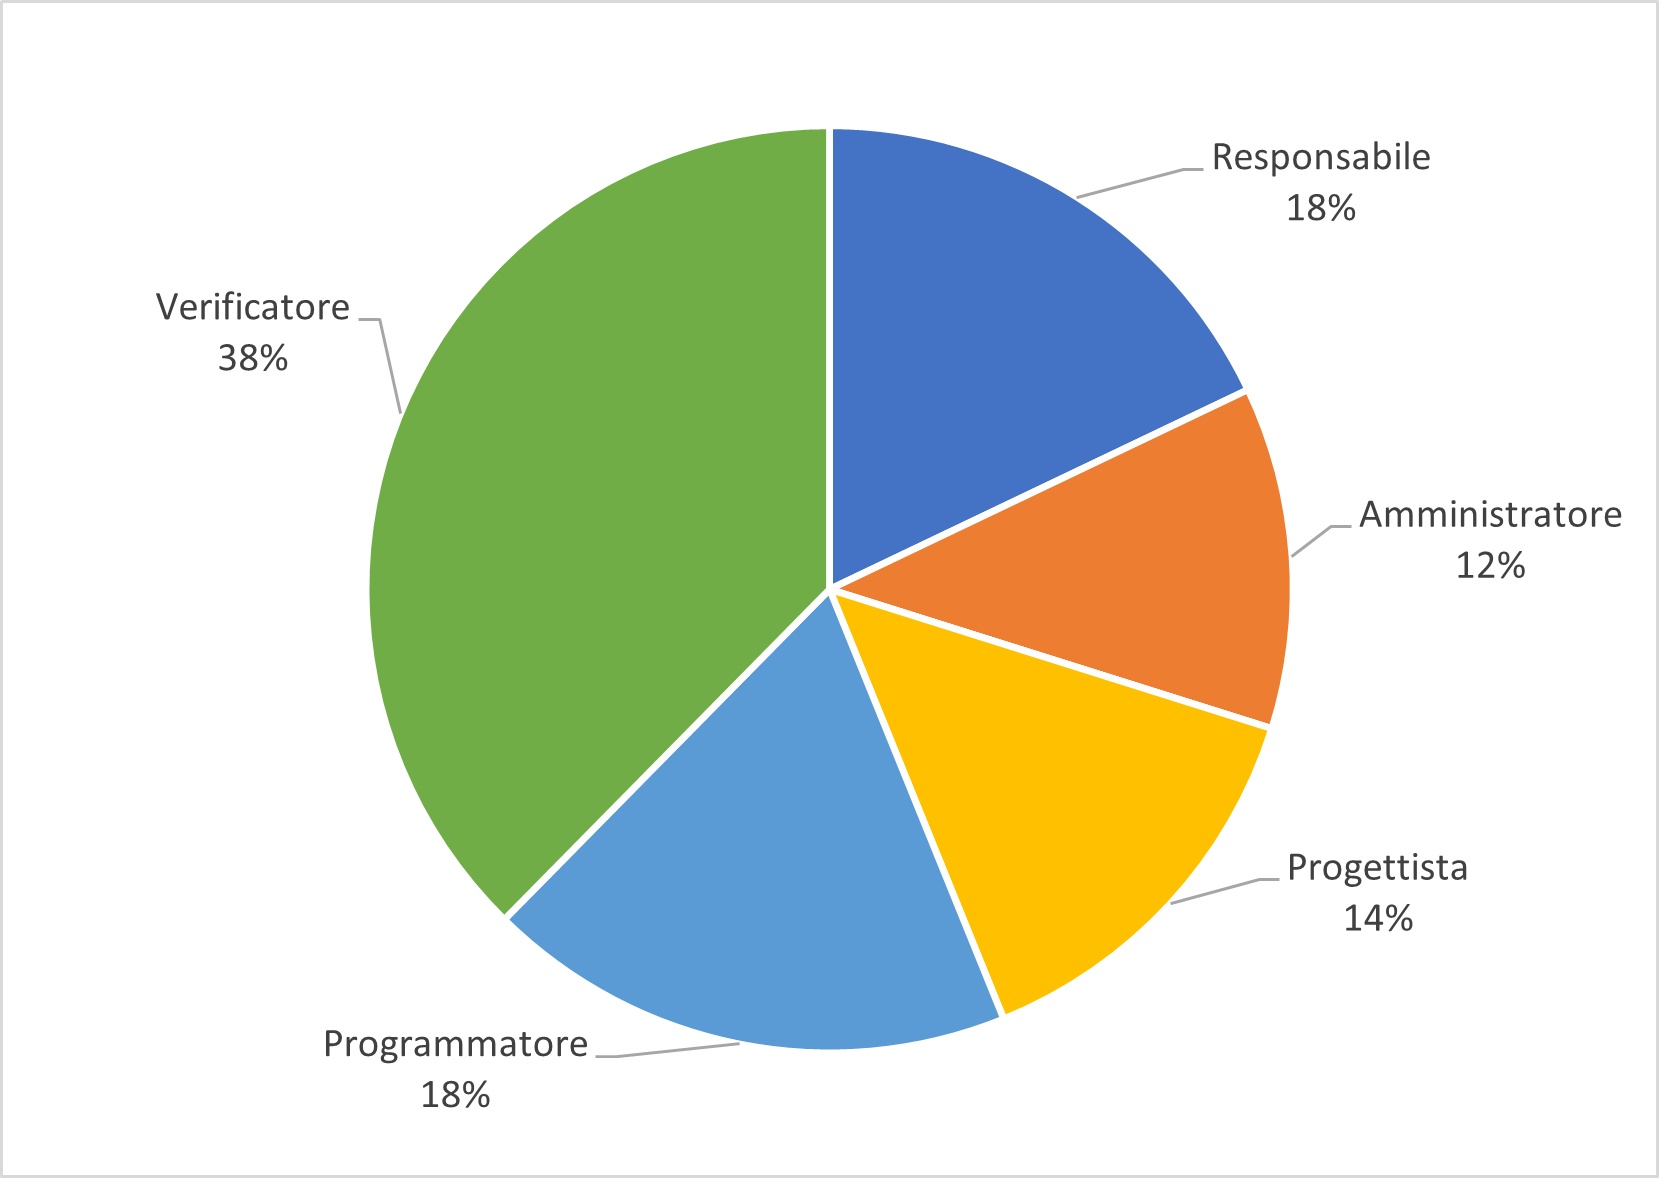
\includegraphics[scale=0.90]{res/Preventivo/Fasi/VerificaIncrementi/tortaFase}\\
\caption{Areogramma della distribuzione economica nella fase di validazione e collaudo}
\end{figure}





